\documentclass[11pt,a4paper]{article}
\usepackage[utf8]{inputenc}
\usepackage[T1]{fontenc}
\usepackage[indonesian]{babel}
\usepackage{lmodern}
\usepackage{geometry}
\usepackage{amsmath,amssymb,booktabs,array,graphicx,float}
\usepackage{microtype}
\usepackage[hidelinks]{hyperref}
\geometry{margin=2.25cm}
\graphicspath{{figures/}}
\newcommand{\R}{\mathbb{R}}
\newcommand{\norm}[1]{\left\lVert #1\right\rVert_2}
\title{Laporan Teknis TK 1 Analisis Numerik\\[3pt]
\large Soal 2: Deteksi Rezim Pasar dan Prediksi Return Saham dengan SETAR}
\author{Kelompok: \underline{\hspace{4cm}}\\[5pt]
Anggota dan NPM: \underline{\hspace{8cm}}}
\date{Semester Gasal 2026/2027}

\begin{document}
\maketitle
\begin{center}
\fbox{\begin{minipage}{0.87\textwidth}
\textbf{Pernyataan integritas.} Dengan ini, kami menyatakan bahwa tugas ini adalah hasil pekerjaan kelompok sendiri.\\[1.5em]
Tanda tangan seluruh anggota: \underline{\hspace{7cm}}
\end{minipage}}
\end{center}

\begin{abstract}
Kami mengestimasi enam parameter model SETAR dua rezim dari 303 harga penutupan saham dengan metode persamaan normal dan QR rotasi Givens. Kedua metode menghasilkan koefisien yang sama hingga presisi numerik pada data ini. Norma residual latih adalah 0.15297705; RMSE latih dan uji masing-masing 0.00883213 dan 0.01196708. QR menghindari pembentukan $A^\mathsf{T}A$, yang memperbesar bilangan kondisi dari 192.61 menjadi 37096.84, tetapi implementasi Givens yang menyimpan matriks ortogonal penuh membutuhkan lebih banyak memori dan operasi. Evaluasi uji menggunakan 103 return yang dihitung sambung dari harga terakhir data latih.
\end{abstract}

\section{Formulasi matriks desain}
Untuk harga penutupan $P_t$, return harian adalah $R_t=(P_t-P_{t-1})/P_{t-1}$. Baris pertama deret return tidak terdefinisi. Dengan ambang $c=0$ dan dua lag, model untuk $t\geq3$ dalam indeks array Python adalah
\begin{equation}
R_t=\begin{cases}
\alpha_1+\phi_{1,1}R_{t-1}+\phi_{1,2}R_{t-2}+\varepsilon_t,& R_{t-1}\geq0,\\
\alpha_2+\phi_{2,1}R_{t-1}+\phi_{2,2}R_{t-2}+\varepsilon_t,& R_{t-1}<0.
\end{cases}
\end{equation}
Definisikan $x=(\alpha_1,\phi_{1,1},\phi_{1,2},\alpha_2,\phi_{2,1},\phi_{2,2})^\mathsf{T}$ dan $b_t=R_t$. Baris matriks desain adalah
\[
A_t=\begin{cases}
(1,R_{t-1},R_{t-2},0,0,0),&R_{t-1}\geq0,\\
(0,0,0,1,R_{t-1},R_{t-2}),&R_{t-1}<0.
\end{cases}
\]
Persoalannya ialah $\min_x\norm{Ax-b}$. Dari 303 harga latih diperoleh 302 return dan $m=300$ observasi lengkap, sehingga $A\in\R^{300\times6}$, $x\in\R^6$, dan $b\in\R^{300}$. Ada 195 baris bullish dan 105 bearish.

Penentuan rezim dan lag selalu memakai return sebelum target. Ini mencegah kebocoran target ke dalam $A$. Pada data uji, return pertama dihitung dari harga pertama uji dan harga terakhir latih, sementara dua lag awal juga memakai riwayat latih. Karena itu seluruh 103 harga uji menjadi 103 target return yang sah; tidak ada parameter yang diestimasi ulang dari data uji.

\section{Isu numerik dan mitigasi}
Kolom intersep berisi 0 atau 1, sedangkan kolom return biasanya berorde $10^{-2}$. Skala kolom yang berbeda serta korelasi antarlag dapat membuat $A$ kurang baik kondisinya. Satu rezim yang sangat jarang muncul juga dapat membuat parameter rezim tersebut sukar diidentifikasi; kedua rezim pada data ini tetap mempunyai jauh lebih banyak observasi daripada tiga parameternya. Return ekstrem dapat mendominasi jumlah kuadrat residual.

Mitigasi yang relevan ialah memeriksa rank dan bilangan kondisi, membangun lag tanpa memakai target, dan menggunakan transformasi ortogonal untuk menghindari kuadrat bilangan kondisi. Jika perlu, kolom prediktor dapat diskalakan sebelum penyelesaian dan koefisien dikonversi kembali ke satuan semula. Pensakalan harus dihitung dari data latih saja. Pada laporan ini koefisien dilaporkan dalam skala return asli.

\section{Persamaan normal}
Syarat stasioner $\norm{Ax-b}^{2}$ menghasilkan
\begin{equation}
A^\mathsf{T}Ax=A^\mathsf{T}b.
\end{equation}
Matriks $6\times6$ dibentuk dari data latih, lalu sistemnya diselesaikan dengan eliminasi Gauss dan \emph{partial pivoting} serta substitusi balik yang diimplementasikan sendiri. Dalam aritmetika eksak, $\kappa_2(A^\mathsf{T}A)=\kappa_2(A)^2$ bila $A$ ber-rank penuh. Untuk data ini, $\kappa_2(A)=192.6054$ dan $\kappa_2(A^\mathsf{T}A)=37096.8440$. Membentuk persamaan normal karena itu berpotensi memperbesar pengaruh pembulatan dan kehilangan digit akurasi, walaupun hasil pada data ini masih sangat dekat dengan QR.

\section{QR dengan rotasi Givens}
Untuk menghilangkan entri $a_{ji}$ di bawah diagonal, ambil $u=a_{ii}$, $v=a_{ji}$, $\rho=\sqrt{u^2+v^2}$, $c=u/\rho$, dan $s=v/\rho$. Matriks $G$ adalah identitas kecuali blok pada baris dan kolom $i,j$:
\begin{equation}
G_{\{i,j\},\{i,j\}}=\begin{pmatrix}c&s\\-s&c\end{pmatrix},\qquad
G\begin{pmatrix}u\\v\end{pmatrix}=\begin{pmatrix}\rho\\0\end{pmatrix}.
\end{equation}
Penerapan seluruh rotasi memberi $R=G_k\cdots G_1A$ dan $Q_{\rm QR}=(G_k\cdots G_1)^\mathsf{T}$, sehingga $A=Q_{\rm QR}R$. Jika variabel program \texttt{Q} menyimpan $G_k\cdots G_1$, ruas kanan yang benar adalah \texttt{d = Q @ b}; lalu selesaikan enam baris pertama $Rx=d$ dengan substitusi balik. Ini adalah orientasi yang dipakai pada perhitungan.

\subsection*{Verifikasi rotasi pertama}
Dua baris pertama matriks desain adalah
\[
\begin{pmatrix}
0&0&0&1&-0.00831972&0.00243800\\
1&0.00737754&-0.00831972&0&0&0
\end{pmatrix}.
\]
Entri subdiagonal pertama adalah $a_{21}=1$, sedangkan $a_{11}=0$. Maka $c=0$, $s=1$, dan blok rotasi pertama adalah $\left(\begin{smallmatrix}0&1\\-1&0\end{smallmatrix}\right)$. Dua baris pertama $G_1A$ menjadi
\[
\begin{pmatrix}
1&0.00737754&-0.00831972&0&0&0\\
0&0&0&-1&0.00831972&-0.00243800
\end{pmatrix}.
\]
Dengan demikian entri $(2,1)$ tepat menjadi nol. Seluruh rotasi berikutnya memakai rumus yang sama.

\section{Perbandingan hasil dan biaya}
\begin{table}[H]
\centering
\caption{Perbandingan pada matriks desain yang sama. Biaya Givens berlaku untuk pembaruan dua baris; RMSE uji memakai 103 return sambung.}
\begin{tabular}{lrr}
\toprule
Ukuran & Persamaan normal & QR Givens\\
\midrule
$\norm{Ax-b}$ & 0.15297705 & 0.15297705\\
RMSE latih & 0.00883213 & 0.00883213\\
RMSE uji & 0.01196708 & 0.01196708\\
Norma selisih koefisien & \multicolumn{2}{c}{$2.44\times10^{-16}$}\\
FLOP teoretis utama & $2mn^2+2mn+2n^3/3$ & $O(mn^2)$\\
Memori tambahan & $O(n^2)$ & $O(m^2)$ jika $Q$ eksplisit\\
\bottomrule
\end{tabular}
\end{table}

\begin{table}[H]
\centering
\caption{Koefisien SETAR hasil kedua metode; selisihnya hanya pada digit pembulatan.}
\begin{tabular}{lrr}
\toprule
Parameter & Persamaan normal & QR Givens\\
\midrule
$\alpha_1$ & 0.00151337 & 0.00151337\\
$\phi_{1,1}$ & 0.17215290 & 0.17215290\\
$\phi_{1,2}$ & 0.16607285 & 0.16607285\\
$\alpha_2$ & -0.00121269 & -0.00121269\\
$\phi_{2,1}$ & -0.36037682 & -0.36037682\\
$\phi_{2,2}$ & -0.10980804 & -0.10980804\\
\bottomrule
\end{tabular}
\end{table}

Untuk $m\times n$ dengan $m\gg n$, pembentukan $A^\mathsf{T}A$ memerlukan sekitar $2mn^2$ FLOP, $A^\mathsf{T}b$ sekitar $2mn$, dan eliminasi $n\times n$ sekitar $2n^3/3$. Givens yang memperbarui hanya dua baris aktif memerlukan $O(mn^2)$ FLOP; pembentukan dan penerapan rotasi pada ruas kanan menambah $O(mn)$. Untuk $m=300,n=6$, ada paling banyak 1779 rotasi; sekitar 48 ribu FLOP diperlukan untuk pembaruan baris dan ruas kanan pada batas atas ini, di luar pembentukan parameter rotasi. Kedua metode berorde $O(mn^2)$ untuk matriks tinggi, dengan konstanta Givens lebih besar.

Jika $A$ disimpan dense, keduanya memakai $O(mn)$ memori dasar. Persamaan normal menambah $O(n^2)$; $A$ berisi 1800 bilangan \texttt{float64} (14.4 kB) dan $A^\mathsf{T}A$ hanya 36 bilangan (288 byte). Implementasi notebook menyimpan $Q$ berukuran $300\times300$ dan membuat $G$ berukuran sama, masing-masing sekitar 720 kB; perkalian dense penuh untuk setiap rotasi juga mahal. Pembaruan langsung dua baris $[A\mid b]$, seperti pada skrip reproduksi laporan, menghindari penyimpanan $Q$ dan menghasilkan solusi yang sama. Keuntungan utama QR ialah stabilitas terhadap pembulatan, bukan jaminan residual yang lebih kecil pada setiap data. Residual dan koefisien yang sama pada kasus ini konsisten dengan kondisi matriks yang belum cukup ekstrem untuk memisahkan hasil kedua metode dalam presisi ganda.

\section{Evaluasi luar sampel dan interpretasi}
RMSE dihitung sebagai $\sqrt{\sum_{t=1}^{N}(R_t-\widehat R_t)^2/N}$. Hasil uji 0.01196708 lebih besar daripada hasil latih 0.00883213, sehingga kesalahan prediksi meningkat di luar sampel. Karena parameter kedua metode praktis identik, akurasi prediksi dan residualnya juga identik pada presisi yang dilaporkan; data ini tidak mendukung klaim bahwa salah satunya lebih akurat secara empiris. QR tetap lebih aman dari sisi stabilitas algoritmik bila kondisi masalah memburuk.

Persamaan estimasi akhirnya adalah
\begin{equation}
\widehat R_t=\begin{cases}
0.00151337+0.17215290R_{t-1}+0.16607285R_{t-2},&R_{t-1}\geq0,\\
-0.00121269-0.36037682R_{t-1}-0.10980804R_{t-2},&R_{t-1}<0.
\end{cases}
\end{equation}
Kedua koefisien lag pada rezim bullish positif, yang sesuai dengan kecenderungan penerusan return sebelumnya pada model. Kedua koefisien lag pada rezim bearish negatif, yang sesuai dengan pembalikan arah bersyarat. Ini adalah interpretasi koefisien model, bukan bukti hubungan sebab-akibat ataupun jaminan kinerja investasi.

\begin{figure}[H]
\centering
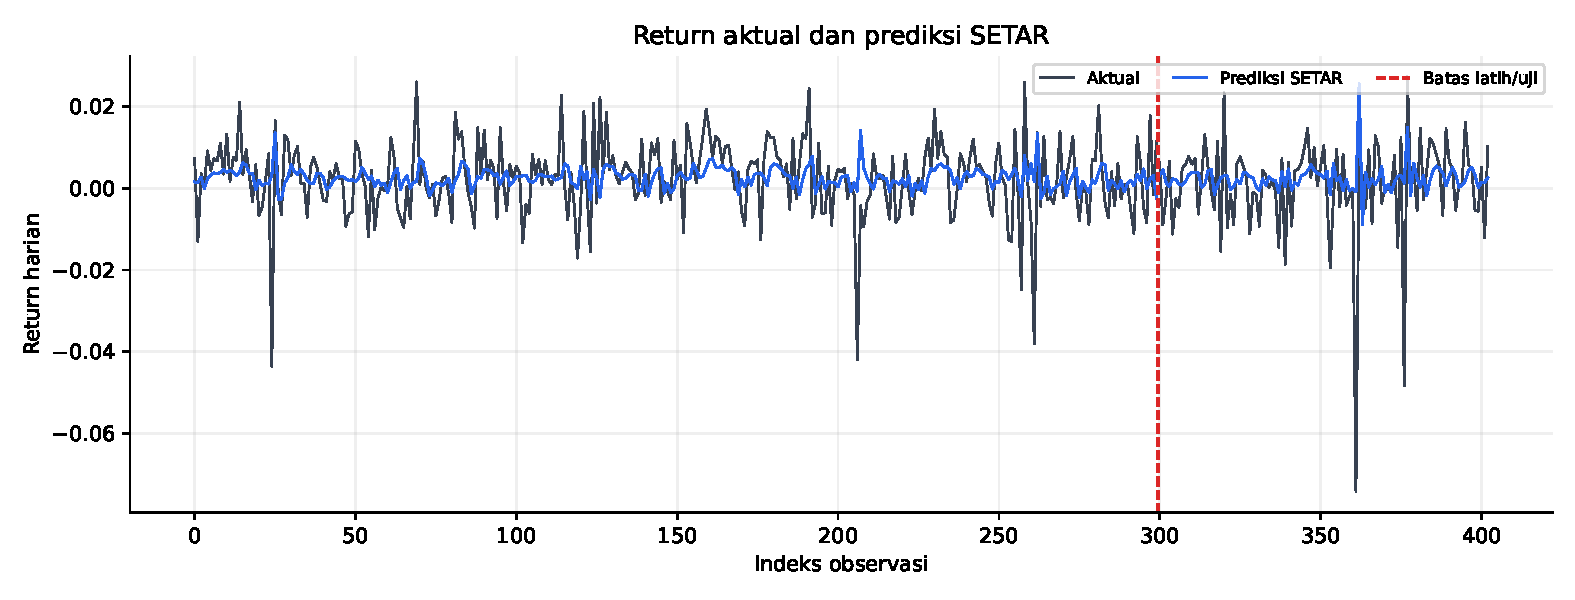
\includegraphics[width=0.82\textwidth]{figures/overlay.pdf}
\caption{Return aktual dan prediksi dari model yang dilatih pada segmen kiri. Garis putus-putus menunjukkan batas latih/uji; indeks uji pertama memakai riwayat harga latih.}
\end{figure}

\begin{figure}[H]
\centering
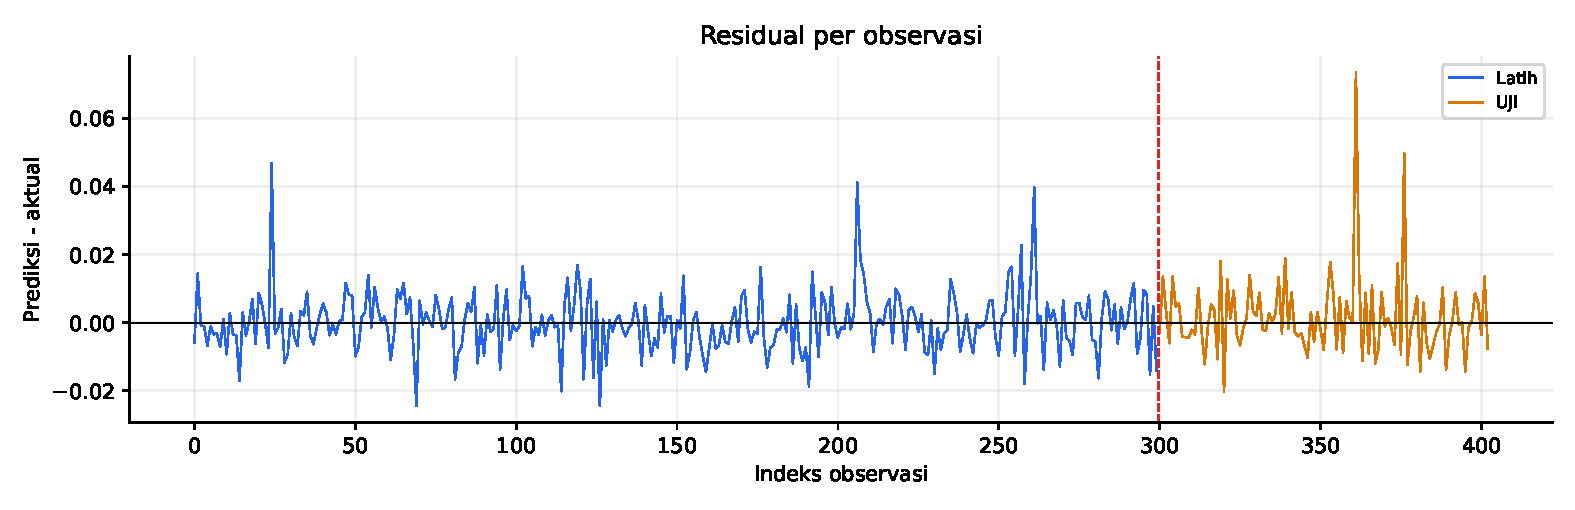
\includegraphics[width=0.82\textwidth]{figures/residuals.pdf}
\caption{Residual prediksi per observasi. Beberapa deviasi besar tetap muncul walaupun parameter diperoleh dengan meminimalkan jumlah kuadrat galat latih.}
\end{figure}

\section{Pengaruh outlier dan kesimpulan}
Fungsi objektif $\sum_t(R_t-\widehat R_t)^2$ memberi bobot kuadrat pada tiap galat. Karena itu kejutan harga ekstrem dapat menaikkan norma residual secara tajam dan menarik koefisien ke arah observasi tersebut. Pada data latih, return absolut terbesar sekitar 0.04357 dan galat prediksi absolut terbesar sekitar 0.04681 (29 Januari 2024). Galat maksimum pada data uji sekitar 0.07347. Plot residual menunjukkan mengapa RMSE uji dapat meningkat meski penyelesaian kuadrat terkecil pada data latih sudah optimal. Analisis sensitivitas yang lebih lengkap dapat membandingkan hasil dengan dan tanpa observasi ekstrem, menggunakan aturan yang ditentukan sebelum melihat data uji.

Kedua solver berhasil menyelesaikan model yang sama dan menghasilkan angka yang identik pada ketelitian pelaporan. Untuk implementasi yang efisien dan lebih tahan terhadap pembulatan, QR Givens sebaiknya diterapkan langsung pada dua baris matriks kerja dan ruas kanan, tanpa membentuk $Q$ atau $G$ dense penuh. Persamaan normal masih layak sebagai pembanding pada data ini, tetapi bilangan kondisinya yang kuadrat perlu diperhatikan jika skala atau korelasi prediktor meningkat.

\end{document}
